\begin{activity} \label{A:9.5.8}  Let $p$ be the plane with equation $z=-4x+3y+4$, whose graph is shown in Figure \ref{F:9.5.Point_to_plane}. (Note that we can always find an equation of this form by expanding the scalar equation and collecting the constant terms). Let $Q = (4,-1,8)$.
\begin{figure}[ht]
\begin{center}
\resizebox{!}{2.5in}{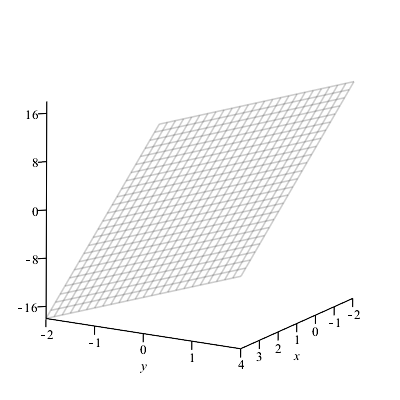
\includegraphics[trim=0cm 0.25cm 0cm 1.5cm, clip]{9_5_Point_to_plane}}
\end{center}
\caption{Graph of $z=-4x+3y+4$.}
\label{F:9.5.Point_to_plane}
\end{figure}
%crop graphics in animate trim=<left> <bottom> <right> <top>, add, clip with \includegraphics
	\ba
	\item Show that $Q$ does not lie in the plane $p$.
	
	
	
	\item Find a normal vector $\vn$ to the plane $p$.
	
	
	
	\item Find the coordinates of a point $P$ in $p$.
	


	\item Find the components of $\overrightarrow{PQ}$. Draw a picture in Figure \ref{F:9.5.Point_to_plane} to illustrate the objects found so far.
	
	
	
	\item Explain why $|\comp_{\vn} \overrightarrow{PQ}|$ gives the distance from the point $Q$ to the plane $p$. Find this distance.
	
	
	
	\ea


\end{activity}
\begin{smallhint}

\end{smallhint}
\begin{bighint}

\end{bighint}
\begin{activitySolution}

\end{activitySolution}
\aftera
